% sample latex/latex2e file with lots of math, tables, figures, etc
% useful for writing papers
% genuine finger-typed files by Christina C. Christara

\documentclass[12pt]{article}
% \documentclass[12pt]{mypaper}

%\linespread{1.1} % for more than single spacing

% take more advantage of the size of paper
\addtolength{\topmargin}{-2cm}
\addtolength{\textheight}{4cm}
\addtolength{\evensidemargin}{-2cm}
\addtolength{\oddsidemargin}{-2cm}
\addtolength{\textwidth}{4cm}

% some standard packages
\usepackage{times}
\usepackage{graphics}
\usepackage{subfigure, epsfig}
\usepackage{rotate}
\usepackage{amssymb}
\usepackage{amsmath}
\usepackage{tikz} % neural networks
\usetikzlibrary{matrix,chains,positioning,decorations.pathreplacing,arrows}


\setlength{\parskip}{3mm}
% convenient abbreviations
\newcommand{\de}{\partial}

\begin{document}
\begin{center}
Proposal - M.Sc. Research Project \\
by \\
Bill (Mufan) Li \\
% M.Sc Candidate \\
Supervised by Professor Jeffrey Rosenthal \\
Department of Statistical Sciences \\
University of Toronto \\
Phone: (416)843-9179\\
Email: {\tt mufan.li@mail.utoronto.ca}\\
\bigskip\large
{\bf Assessing GPA Measures From a Collaborative Filtering
Perspective}
\end{center}

Recent developments in machine learning have made significant 
contributions to a wide range of fields that are not 
traditionally considered data science.
Notably the Netflix competition have attracted a collective
effort in developing models that greatly improved prediction
of movie ratings by different users,
creating the best movie recommendation system at the time [1].
This research project aims to apply the machine learning
techniques in analyzing the student grade dataset in [2].
This analysis provides further insight towards student behavior for
course selection, inference on a student's potential grade
in courses not selected, and ultimately estimation
of an equivalent grades by inferencing on the same set of courses.
The potential application of the results include but limited to
tuning difficulty of courses for fair grading, 
predicting demand of courses,
and improving admission selection process.

Inference on missing data in the
student grade dataset falls directly under a collaborative
filtering problem, where a value or grade is assigned for
some matches of students and courses.
The greatest difficulty of this type of problem is the sparsity
of data, where each student can only take a small subset of 
courses, leaving majority of potential course grades missing.
Additionally, data is not even distributed among courses, 
where some courses can have few attendance.
Therefore, common methods of inference will be difficult
to perform with this type of problem.
That being said, matrix factorization and restricted Boltzmann
machines have been highly effective at collaborative filtering.
This project intends to investigate these two techniques and
the respective extensions with the student grade dataset.

The most basic matrix factorization (MF) method
known as singular value decomposition (SVD),
where a large low-rank matrix 
is decomposed into a product of two low-rank matrices.
Specifically for this problem, 
suppose there are $M$ students and $N$ courses,
then we define $\mathbf{A} \in \mathbb{R}^{M \times N}$ 
as the matrix of grades,
where $A_{ij}$ corresponds to the grade of 
student $i$ and course $j$.
We then seek two low-rank matrices 
$\mathbf{U} \in \mathbb{R}^{M \times d}$ 
and $\mathbf{V} \in \mathbb{R}^{N \times d}$ such that
%
\begin{equation}
	\mathbf{A} \approx \mathbf{UV}^\top .
\end{equation}
%
This is called a rank $d$ approximation of $\mathbf{A}$.
Note the value $A_{ij}$ is the dot product of
the $i$th row of $\mathbf{U}$ and 
the $j$th row of $\mathbf{V}$.
The row vectors may be interpreted as features,
i.e. row $i$ of $\mathbf{U}$ contains all the information
of student $i$.

The best rank $d$ approximation is the decomposition
that minimizes the Frobenius norm of the difference
$\left\Vert \mathbf{A - UV}^\top \right\Vert$,
defined by the square root of the
sum of squares of its entries.
In the case of collaborative filtering,
the Frobenius norm is not computed for missing entries.
By the Eckart-Young Theorem, given a best rank $k-1$ approximation
of $\mathbf{U}$ and $\mathbf{V}$, 
a best rank $k$ approximation is obtained by adding
a column to both $\mathbf{U}$ and $\mathbf{V}$
such that the product minimizes 
the Frobenius norm of the difference.

This key result allows for iterative computation of 
$\mathbf{U}$ and $\mathbf{V}$,
reducing the complexity significantly.
One approach, known as alternating least squares (ALS),
fixes the column of interest of $\mathbf{U}$ 
while using least squares
to fit the column of $\mathbf{V}$, 
then fixing $\mathbf{V}$ to fit $\mathbf{U}$,
and alternates until convergence.
The other approach calculates the gradient of
the Frobenius norm
with respect to all elements of $\mathbf{U}$ and $\mathbf{V}$,
and perform steepest descent until convergence.
While the optimization problem is non-convex,
both approaches have been proven to reach satisfactory 
local minima [1].

The greatest advantage of SVD is the simplicity of 
both implementation and inference,
where each missing value $A_{ij}$ is just 
the dot product of two row vectors of $\mathbf{U}$
and $\mathbf{V}$.
One extension of SVD is by defining
a probabilistic distribution using the matrix product
instead of directly using the value [3].
Probabilistic MF allows the incorporation of student or course 
specific information with parameters of the distribution.
For example, a student's GRE score cannot be easily
used by SVD, but not can be directly used by a
probabilistic model.

On the other hand, restricted Boltzmann machines (RBM) is a
completely different approach to the problem.
Similar to probabilistic MF, RBM can easily incorporate
student specific information within the model.
A RBM is a Markov random field in the form of a bipartite graph,
where the joint probability follows a Boltzmann type distribution.

\def\layersep{2.5cm}

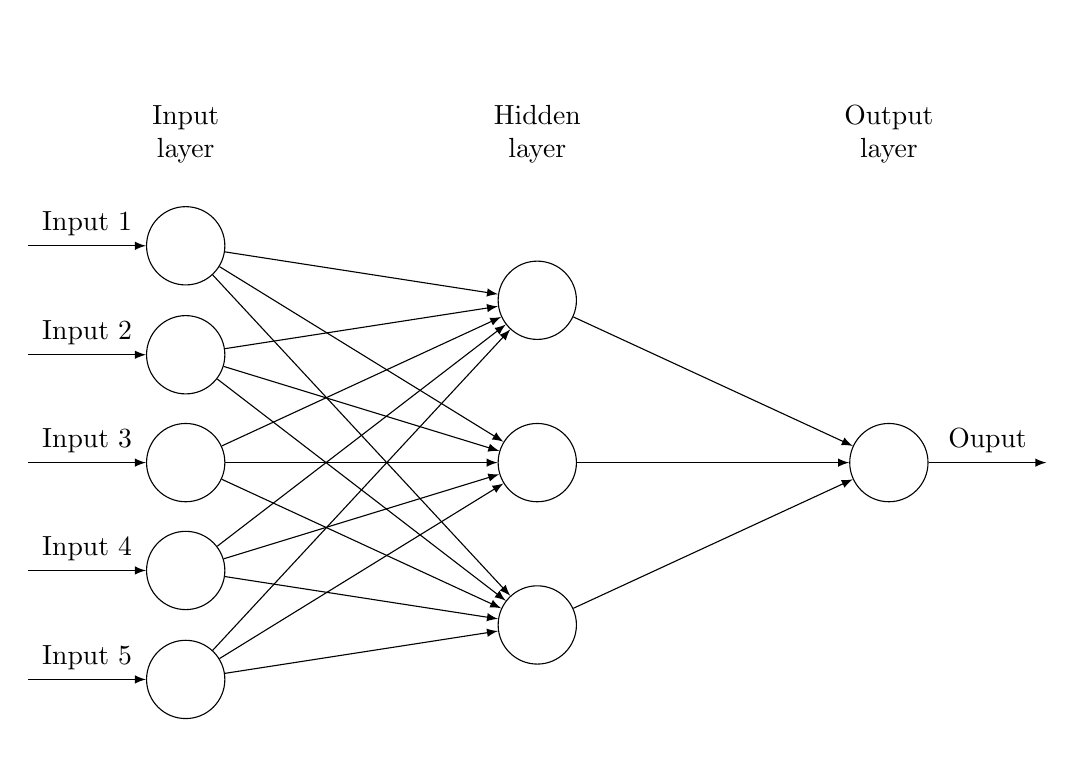
\begin{tikzpicture}[
plain/.style={
  draw=none,
  fill=none,
  },
net/.style={
  matrix of nodes,
  nodes={
    draw,
    circle,
    inner sep=10pt
    },
  nodes in empty cells,
  column sep=2cm,
  row sep=-9pt
  },
>=latex
]
\matrix[net] (mat)
{
|[plain]| \parbox{1.3cm}{\centering Input\\layer} & |[plain]| \parbox{1.3cm}{\centering Hidden\\layer} & |[plain]| \parbox{1.3cm}{\centering Output\\layer} \\
& |[plain]| \\
|[plain]| & \\
& |[plain]| \\
|[plain]| & |[plain]| \\
& & \\
|[plain]| & |[plain]| \\
& |[plain]| \\
|[plain]| & \\
& |[plain]| \\
};
\foreach \ai [count=\mi ]in {2,4,...,10}
  \draw[<-] (mat-\ai-1) -- node[above] {Input \mi} +(-2cm,0);
\foreach \ai in {2,4,...,10}
{\foreach \aii in {3,6,9}
  \draw[->] (mat-\ai-1) -- (mat-\aii-2);
}
\foreach \ai in {3,6,9}
  \draw[->] (mat-\ai-2) -- (mat-6-3);
\draw[->] (mat-6-3) -- node[above] {Ouput} +(2cm,0);
\end{tikzpicture}

The bipartite graph structure creates two layers without
internal connections.
One layer, called the visible layer, contain the 
observed values of grades for a specific student.
These nodes are connected to the other layer, called the hidden layer,
with symmetrical weighted connections.

Suppose the graph have $N$ visible nodes and $M$ hidden nodes,
with each visible node denoted $v_i$, hidden nodes denoted $h_j$, 
weights between two nodes $w_{ij}$,
and $b_i$ and $a_j$ be bias parameters.
Let $\theta = \{ w_{ij},a_j,b_i \} \; \forall i,j$,
$\mathbf{v} = {v_i} \; \forall i$,
and $\mathbf{h} = {h_j} \; \forall j$ denote the vectors.
Additionally, we take the simplest case where
all nodes take binary values, i.e. $v_i, h_j \in \{0,1\}$,
although this can be easily extended to a larger domain.
We can then define the energy function for the graph:
%
\begin{equation}
    E(\mathbf{v},\mathbf{h}|\theta) = 
        - \displaystyle\sum_{i=1}^N \displaystyle\sum_{j=1}^M
             w_{ij} v_i h_j 
        - \displaystyle\sum_{i=1}^N b_i v_i
        - \displaystyle\sum_{i=j}^M a_j h_j
\end{equation}
%
The joint distribution for the graph is then defined
by the Boltzmann distribution:
%
\begin{equation}
    P(\mathbf{v},\mathbf{h}|\theta) = 
        \frac{\exp\left[-E(\mathbf{v},\mathbf{h}|\theta)\right]}
        {\mathcal{Z}}
\end{equation}
%
where $\mathcal{Z}$ is the partition function normalizing
the distribution.
After marginalizing over the hidden nodes $\mathbf{h}$, 
we can find the gradient of the likelihood function
with respect to the parameters $\theta$
to perform steepest descent optimization.
Finding the gradient requires the use of Gibbs sampling,
although [4] describes that the approximate gradient
after few iterations of Gibbs sampling is sufficient
for optimization.
%
% \begin{equation}
%     \frac{\de P(\mathbf{v}|\theta)}{\de w_{ij}} = 
%         \mathbb{E}_{\text{data}} (v_i h_j) -
%         \mathbb{E}_{\text{model}} (v_i h_j)
% \end{equation}
%
% where $\mathbb{E}_{\text{data}}$ refers to expectation 
% of observing the case within data,
% and $\mathbb{E}_{\text{model}}$ is the expectation of 
% the current model with parameters $\theta$.
% Instead of using Gibbs sampling until convergence to find 
% $\mathbb{E}_{\text{model}}$, 
% [4] uses $k$ iterations for a very good approximation
% of the gradient.
% This method is referred to contrastive divergence (CD) by the 
% authors in [4], where CD-$k$ refers to $k$ iterations
% used in Gibbs sampling.
% As a result, we have a very good algorithm optimize the
% RBM for likelihood.

To perform inference on a missing grade value,
one simply include an additional ``visible'' node $v_p$,
where the value is not known, 
but can be determined by the energy function:
%
\begin{equation}
% \begin{aligned}
    P(v_p|\mathbf{v}) \propto
        \displaystyle\sum_{\mathbf{h}} 
        \exp[-E(v_p,\mathbf{v},\mathbf{h})]
    = \prod_{j=1}^M \left( 1 + 
        \exp\left[\sum_{i=1}^N w_{ij} v_i\right]
        \right)
% \end{aligned}
\end{equation}



\medskip
\noindent
{\bf References}

[1] A. Feuerverger, Y. He and S. Khatri
Statistical Significance of the Netflix Challenge
Statistical Science, 27:2, 2012, pp. 202-231

[2] M. Bailey, J. Rosenthal and A. Yoon
Grades and incentives: assessing competing grade point 
average measures and postgraduate outcomes
Studies in Higher Education, 2014
DOI: 10.1080/03075079.2014.982528

[3] Probabilistic Matrix Factorization

[4] Restricted Boltzmann Machine

\end{document}






